\documentclass{article}
\usepackage{graphicx} % Required for inserting images
\usepackage{pgf}
\usepackage{lmodern}
\usepackage{import}
\usepackage{booktabs}
\usepackage{tabu}
\usepackage{float}
\usepackage[hidelinks]{hyperref}
\usepackage{amsmath}
\usepackage{amsfonts}
\usepackage[margin=1in]{geometry}
\usepackage{pythonhighlight}

\setlength{\parskip}{1em}
\setlength{\parindent}{0em}

\title{GYRO REPORT}
\author{Toby Nguyen - z5416116}
\date{May 2024}

\begin{document}
\begin{center}
    \huge{RLC Circuits} \\[10pt]
    \large{Toby Nguyen - z5416116}
\end{center}
\tableofcontents
\newpage
\section{Introduction}
\subsection{Setup}
The RLC circuit is an electrical circuit consisting of a resistor (R), 
an inductor (L), and a capacitor (C), connected in series or in parallel.
The L and C components forms a harmonic oscillator for current. The resistor 
dampens these oscillations, reducing the peak resonant frequency. The most 
basic configuration of these components is shown below in Figure 
\ref{fig:circuit1} with an AC input voltage in series.

\begin{figure}[H]
    \centering
    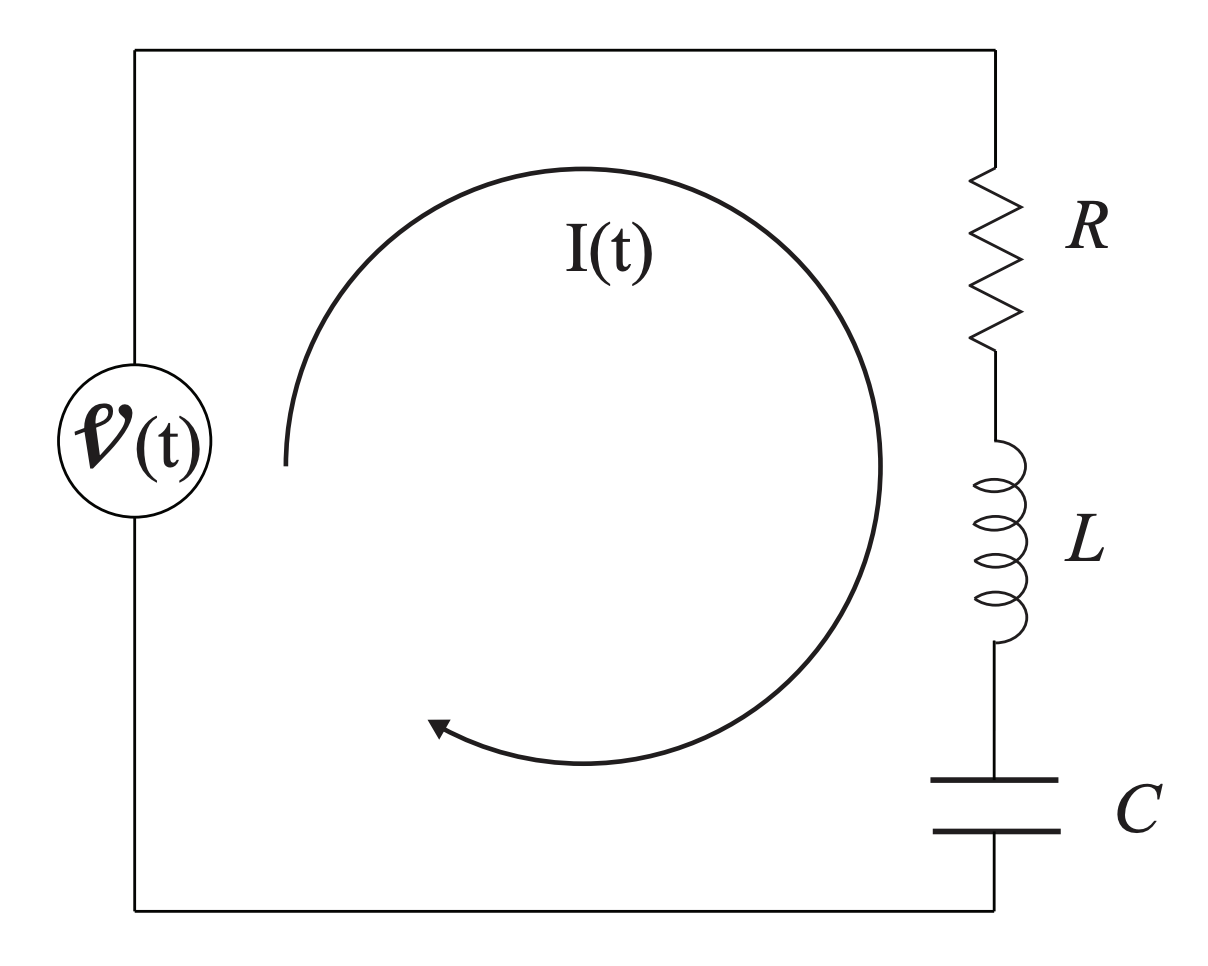
\includegraphics[width=0.5\textwidth]{circuit.png}
    \caption{AC circuit consisting of a voltage source in series with 
    a resistor, an inductor and a capacitor.}
    \label{fig:circuit1}
\end{figure}

\subsection{Kirchhoff's Laws}
Kirchhoff's voltage law states that the directed sum of the potential
differences around any closed loop is zero,
\begin{equation}
    \sum_{i=1}^{n} V_i = 0
\end{equation}
where i is the ith component out of n numbered components. In Figure 
\ref{fig:circuit1}, the voltage at the battery source is taken as positive
so the voltages at each of the 3 RLC components will be taken as negative.
Rearranging gives,
\begin{equation}
    V(t) = V_{R} + V_{L} + V_{C}.
\end{equation}

The voltage drop across the resistor is given by Ohm's law $V_{R}=I(t)R$.

Inductance is defined as the ratio of magnetic flux linkage generated by a 
given current,
\begin{equation}
    \begin{split}
    L &= \frac{\Phi_B}{I} \\
    \Phi_B &= LI.
    \end{split}
\end{equation}

Changes in current through an inductor will create a change in magnetic 
flux and by Faraday's law of induction, will induce an electromotive force
$\mathcal{E}$. Lenz's law states that the induced voltage will be directed
to oppose the original change in flux, hence the negative sign,

\begin{equation}
    \mathcal{E} = -\frac{d\Phi_B}{dt}.
\end{equation}

Substituting Eqn. 3,

\begin{equation}
    \begin{split}
        \mathcal{E} &= -\frac{d}{dt}(LI) \\
        &= -L\frac{dI}{dt}.
    \end{split}
\end{equation}

However, since the voltage drop is taken as positive, the negative sign can
be dropped,
\begin{equation}
    V_L = L\frac{dI}{dt}.
\end{equation}

Lastly, the voltage drop across the capacitor is simply the ratio between the 
charge across the capacitor divided by its capacitance,
\begin{equation}
    V_C = \frac{q}{C}.
\end{equation}

Combining all these equations for the RLC componenets, the following can be 
obtained,
\begin{equation}
    V(t) = I(t)R + L\frac{dI(t)}{dt} + \frac{q}{C}.
\end{equation}
\subsection{RLC Transient Response}
A RLC Transient Response is defined as the temporary change from equilibrium,
due to an external excitation, that will disappear or dampen with time. 
Consider the RLC circuit in Figure \ref{fig:circuit2}, that is suddenly 
disconnected from its voltage supply by opening a switch.

\begin{figure}[H]
    \centering
    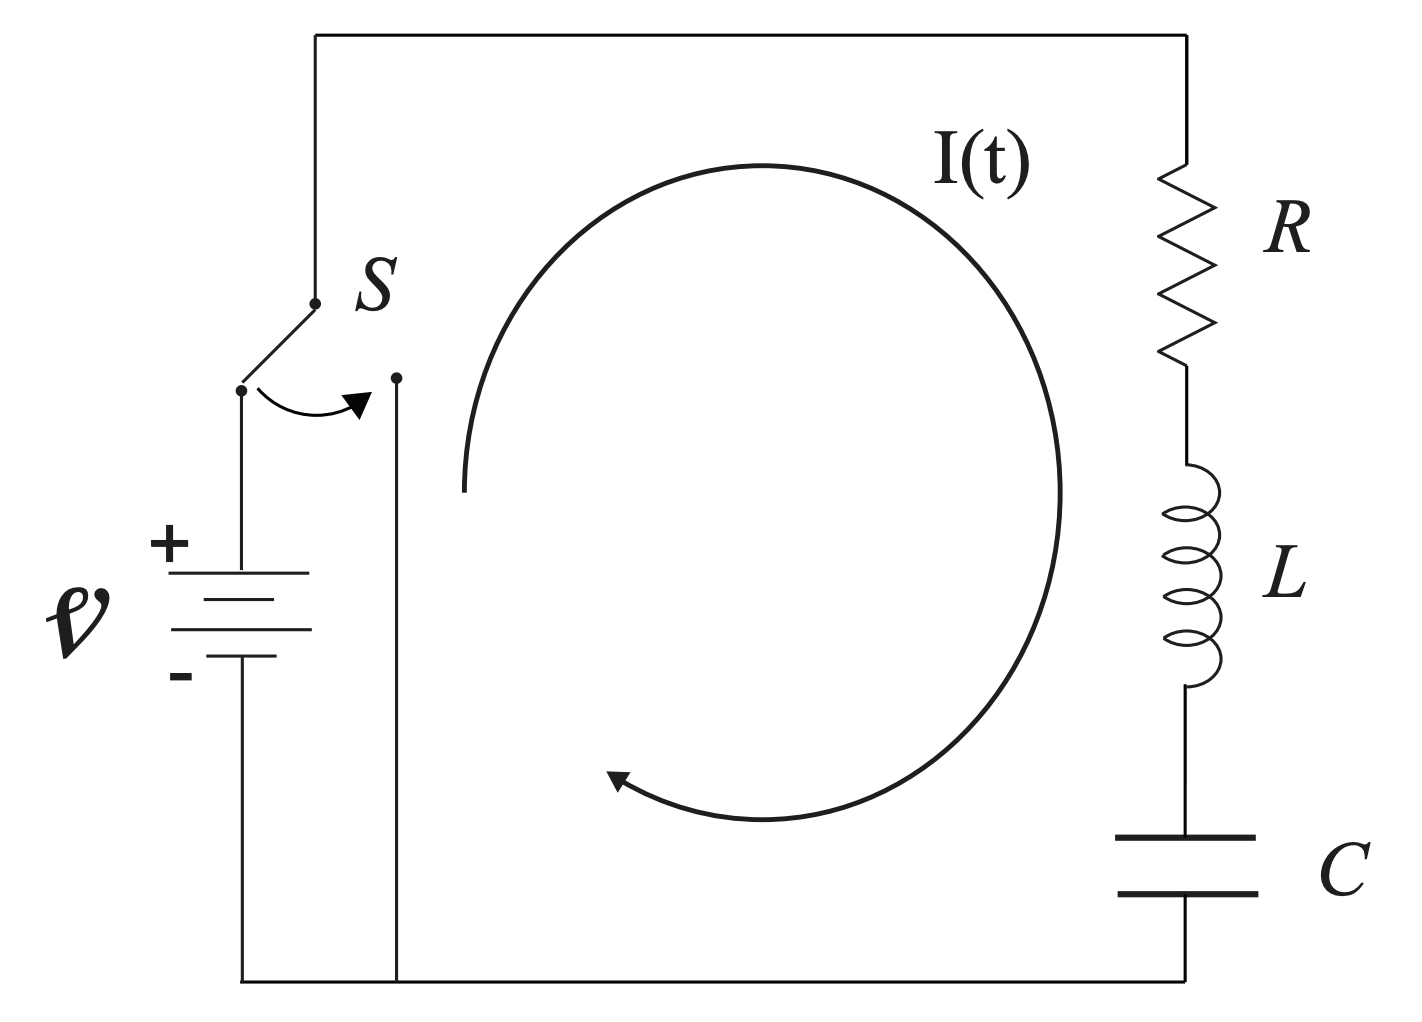
\includegraphics[width=0.5\textwidth]{circuit1.png}
    \caption{Same circuit as before except now it is subject to an 
    instantaneous voltage change when the switch is opened.}
    \label{fig:circuit2}
\end{figure}

Assuming the voltage goes to zero when the switch is open and expressing 
current as the time derivative of charge gives,

\begin{equation}
    0 = R\frac{dq}{dt}+L\frac{d^2q}{dt^2}+\frac{q}{C}.
\end{equation}

The solution is calculated in Appendix \ref{d1}, but is given as,
\begin{equation}
    q(t) = (Ae^{i\omega_nt}+Be^{-i\omega_nt})e^{\frac{-Rt}{2L}}
\end{equation}

with natural frequency,
\begin{equation}
    \omega_n = \sqrt{\frac{1}{LC}-\frac{R^2}{4L^2}}.
\end{equation}

Assuming $A=B^{*}$ and charge $q_0$ at $t=0$, from Appendix \ref{d1},
\begin{equation}
    q = q_0e^{\frac{-Rt}{2L}}\cos{\left(\omega_nt-\delta\right)}.
\end{equation}

This charge can be observed experimentally by measuring the voltage
across the capacitor,
\begin{equation}
    V_c(t) = \frac{q(t)}{C}.
\end{equation}

Experimentally, the resistance will be set to 5 ohms, creating an
underdamped circuit, ie.
\begin{equation}
    \frac{1}{LC} \gg \frac{R^2}{4L^2}.
\end{equation}

Therefore,
\begin{equation}
    \omega_n \sim \omega_0 = \frac{1}{\sqrt{LC}}.
\end{equation}

Defining the damping coefficient, $k=\frac{R}{2L}$ and the period
$T = \frac{2\pi}{\omega_0}$, the amplitude at $nT$, where $n \in 
\mathbb{Z}^{+}$, after $t_0$,
\begin{equation}
    V_n=V_0e^{-k(nT-t_0)}.
\end{equation}

Note here that the cosine term is dropped since only the decaying 
exponential is important in measuring k.

\subsection{RLC Steady-State Response}
After the transient response, i.e once all transient effects have
died out, the system will settle into a steady state. Now assume 
a driving voltage,
\begin{equation}
    V = V_0\cos{\omega t}
\end{equation}
is applied at frequency $\omega$, not necessarily equal to $\omega_n$.

Assume that for $V(t) = V_0e^{i\omega t}$, after transients have passed,
$I(t) = \tilde{I}_0e^{i\omega t}$, where $\tilde{\omega}_0$ is possibly
a complex constant.

Taking the time derivative of Eqn. (8), and substituting,
\begin{equation}
    \begin{split}
        \frac{dV}{dt}&=R\frac{dI}{dt}+L\frac{d^2I}{dt^2}+\frac{I}{C} \\
        i\omega V_0 e^{i\omega t} &=[i\omega R - \omega^2 L + 
        \frac{1}{C}]I_0e^{i\omega t} \\
        V_0 e^{i\omega t} &= \tilde{Z} I_0 e^{i\omega t},
    \end{split}
\end{equation}
where complex impedance is defined as,
\begin{equation}
    \begin{split}
        \tilde{Z} &= R + i\omega L + \frac{1}{i\omega C} \\
        &= R + i(\omega L - \frac{1}{\omega C}).
    \end{split}
\end{equation}

Electrical impedance is the opposition to alternating current
presented by the combined effect of resistance and reactance, $X$, 
in a circuit,

\begin{equation}
    Z = R + iX
\end{equation}

It can be thought of as the AC circuit form of
resistance, possessing both a magnitude and phase.

Reactance is the opposition presented to alternating current
by inductance and capacitance,

\begin{equation}
    \begin{split}
        X &= X_L + X_C \\
        &= \omega L - \frac{1}{\omega C},
    \end{split}
\end{equation}

where $X_L$ is inductive reactance and $X_C$ is capacitive
reactance.

Converting Eqn. (19) into polar coordinates,
\begin{equation}
    \tilde{Z} = |Z|e^{i\theta}
\end{equation}

where,
\begin{equation}
    \begin{split}
    |Z| &= \sqrt{R^2+X^2} \\
    &=\sqrt{R^2+(\omega L - \frac{1}{\omega C})^2}   
    \end{split}
\end{equation}

and,

\begin{equation}
    \theta = \tan^{-1}{\left(\frac{\omega L - \frac{1}{\omega C}}{R}\right)}.
\end{equation}

Thus the complex current is,
\begin{equation}
    I(t) = \frac{V_0}{|Z|}e^{i\left(\omega t - \theta \right)},
\end{equation}

and the real current as,
\begin{equation}
    I(t) = \frac{V_0}{|Z|}\cos\left(\omega t - \theta\right).
\end{equation}

\subsubsection{Resonance}
The minimum impedance occurs when $X_C = X_L$, only occuring at
a singular resonance frequency. When $X = 0$, the impedance is 
only $R$, $|Z| = R$, and $\theta = 0$. Consequently,
\begin{equation}
    \omega^2 = \omega_0^2 = \frac{1}{LC}.
\end{equation}

The maximum current passing through the circuit is then,
\begin{equation}
    I_{max} = \frac{V_0}{R}.
\end{equation}

The quality or Q-factor is a metric that quantifies the frequency response 
of a circuit. It represents the ratio of the energy stored to the energy 
dissipated per cycle by the circuit. It is defined as,

\begin{equation}
    Q = \frac{\omega_0 L}{R} = \frac{1}{R}\sqrt{\frac{L}{C}}.
\end{equation}

\section{Aim}
The aim of this experiment is to study the transient and steady-state 
response of simple electrical circuits. Ultimately, determining the 
constants for dampening, k, and period of oscillation, T, for a transient
response from the circuit and the Q-factor, Q, bandwidth, $\Delta \omega$,
and resonant frequency, $\omega_0$ from driven steady-state responses of the 
circuit.

\section{Method}
\subsection{Setup} \label{constants}
The resistor has a variable resistance but is normally set on 5 $\Omega$.
Ideally, this would be the only source of resistance but due to the design 
and wiring in the inductor and capacitor, it can be found that this is not 
true experimentally. The resistance of the inductor was found to be 10 $\Omega$
and the capacitor was found to be 7 $\Omega$, making the total resistance of
the RLC circuit to be 22 $\Omega$.

The inductor has an inductance of 3.186 mH.

The capacitor has a constant capacitance of 48.5 nF.

\subsection{RLC Transient Response}
The circuit used to excite the damped RLC circuit is shown in Figure 
\ref{fig:circuit3}. A signal generator set with a square wave is connected
to the diode which acts like a valve, allowing current to easily flow in 
one direction whilst resisting current coming from the other direction.
The signal generator provides pulses of current at a set frequency, $f$,
with a 50$\%$ duty cycle.


\begin{figure}[H]
    \centering
    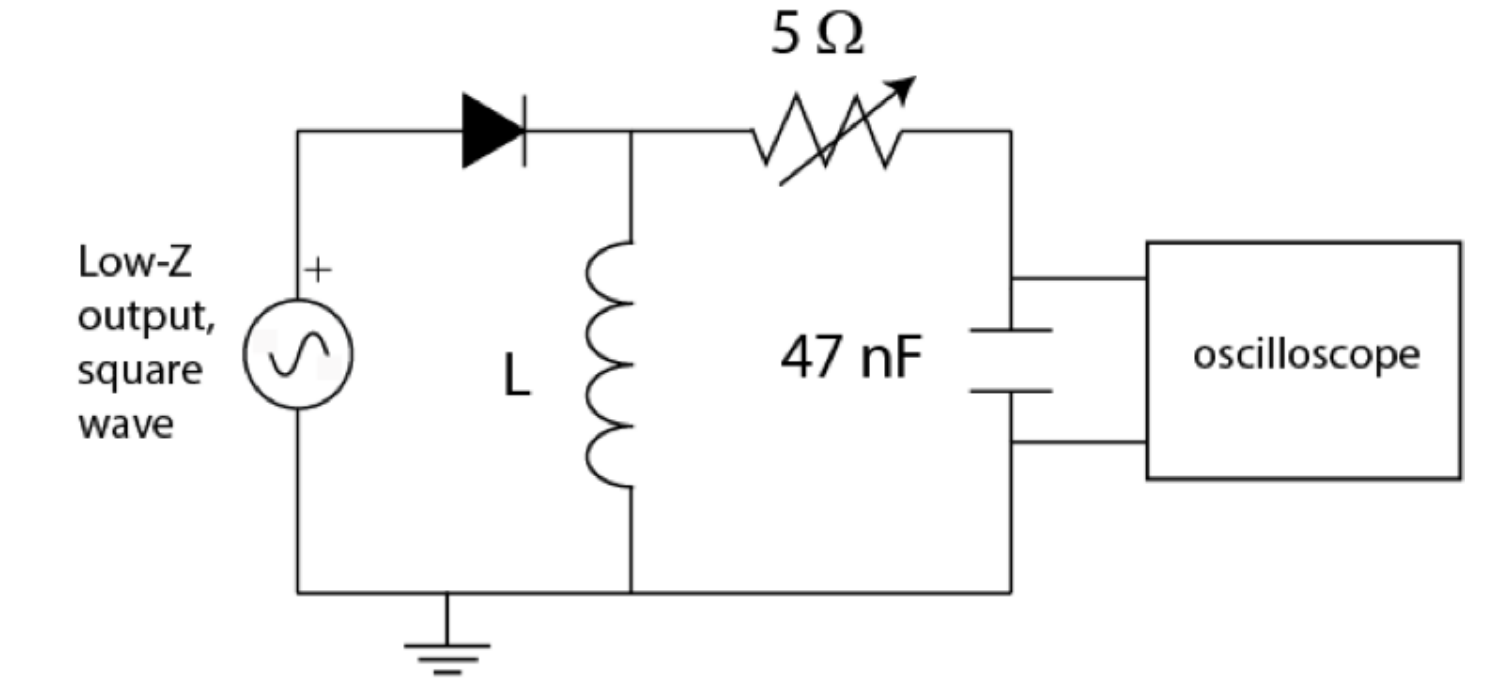
\includegraphics[width=0.5\textwidth]{circuit2.png}
    \caption{Diagram of experimental setup consisting of a diode, variable
    resistor, capacitor, oscilloscope and inductor.}
    \label{fig:circuit3}
\end{figure}

These current oscillations are monitored using an oscilloscope connected 
across the capacitor. These oscillations will dampen due to the inductor 
and resistor in the circuit connected in parallel and series respectively.

In an ideal world, the total resistance is only determined by the resistor
however practically, the inductor and capacitor will contribute a 
non-negligible amount. To find the resistance of the inductor or DC 
resistance (DCR) of the inductor and the resistance of the capacitor or its
equivalent series resistance (ESR), a multimeter set to measuring resistance
will be put in parallel to each component to the circuit.

In this experiment, the coefficient k needs to be determined so
Eqn. (16) must be used, dropping the $t_0$ and substituting in $V_0$,

\begin{equation}
    V_n=V_0e^{-k(nT)}
\end{equation}

where $V_0$ is the initial peak voltage after the transient starts.
The oscilloscope measures the peak voltage for each nth oscillation
and its period. So taking the natural log of $V_n$ and rearranging 
for kT,
\begin{equation}
        \ln(\frac{V_n}{V_0}) =-(kT)n.
\end{equation}

Dividing the gradient of this line graph will produce a value for k.
As with most line graphs, 10 data points is ideal to gauge a 
relationship, so aim for 10 peak to peak cycles.

\subsection{RLC Steady State Response}

The configuration for the second part of the experiment is shown in 
Figure \ref{fig:circuit4}. Like before, the resistor is set to 5 
$\Omega$ and the input voltage limited at 1 V for each frequency.

\begin{figure}[H]
    \centering
    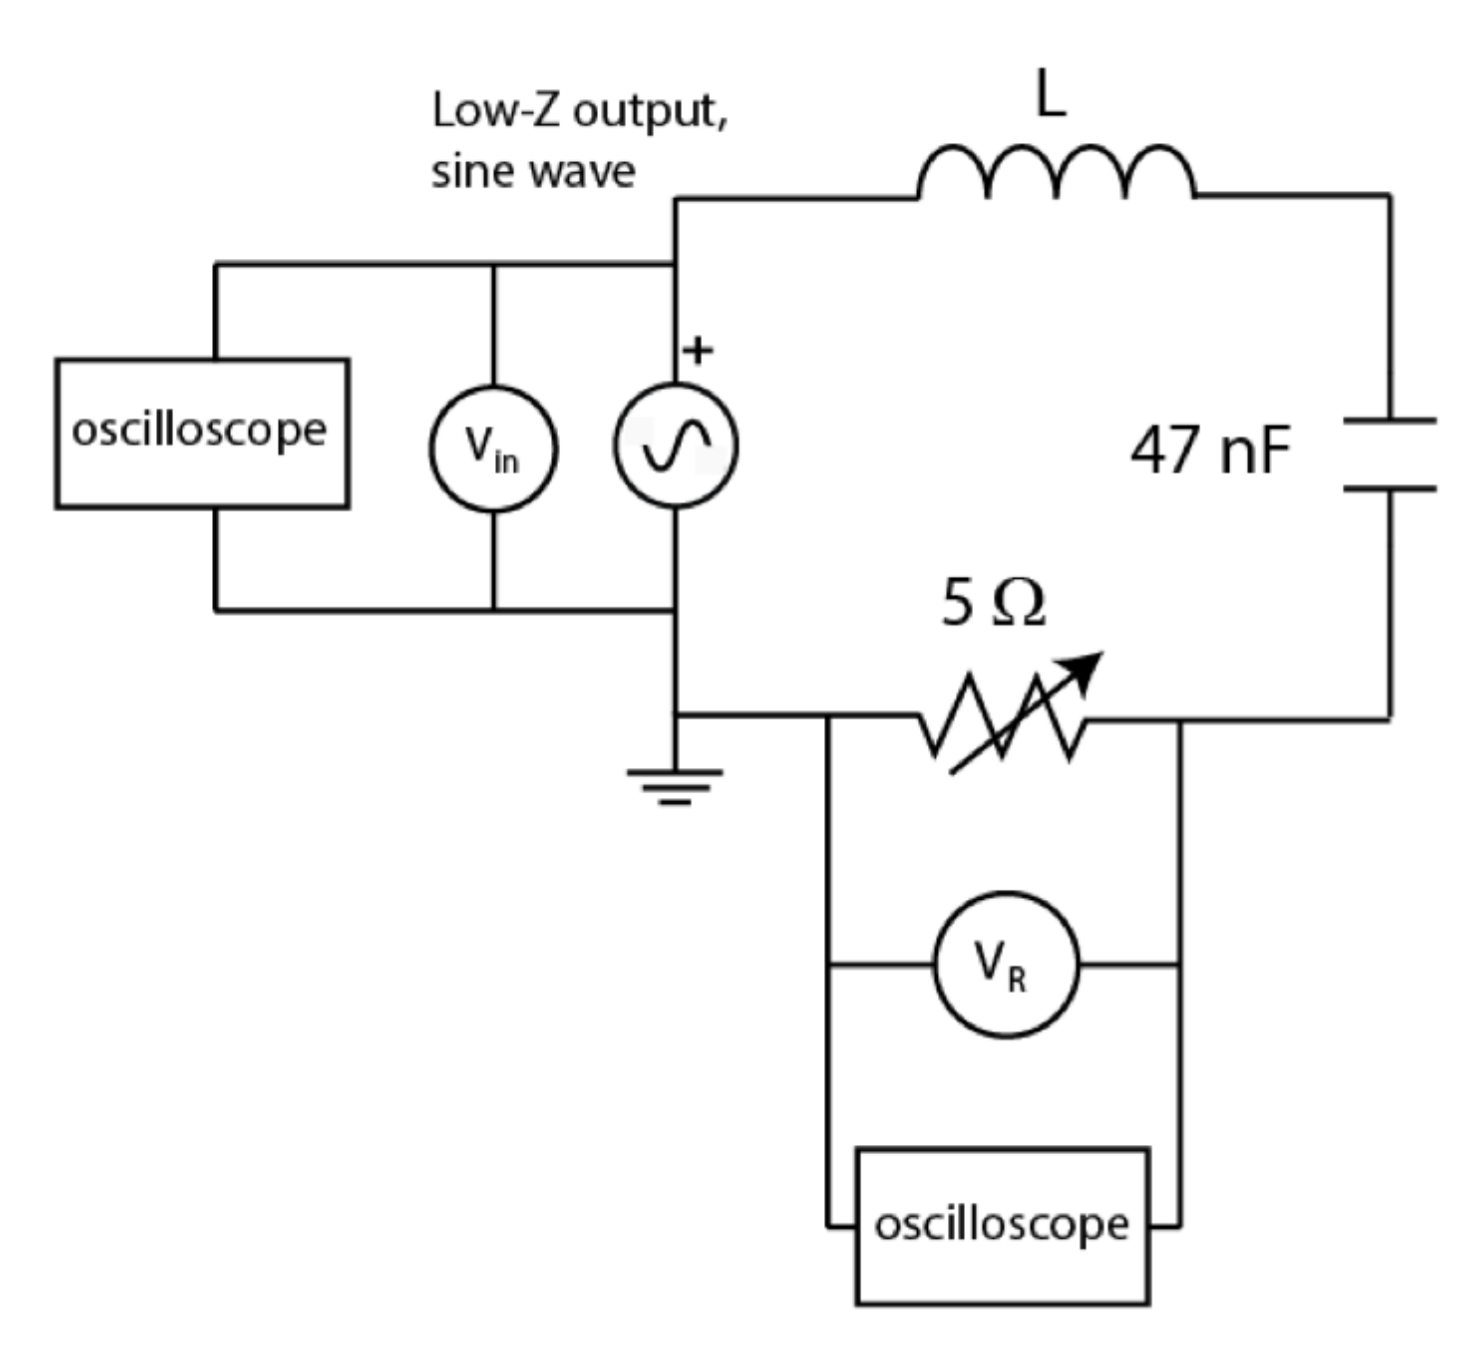
\includegraphics[width=0.5\textwidth]{circuit3.png}
    \caption{A driven RLC oscillator circuit.}
    \label{fig:circuit4}
\end{figure}

The first step is to find the resonant frequency. The quickest 
method is to observe the oscilloscope over the capacitor and 
change the frequency until the peak voltage is achieved. The 
frequency that causes the peak voltage will be the resonant 
frequency. The next step is to closely follow the behaviour of
the system around the peak.

The bandwidth of the circuit can be found by finding the voltage
at the circuit's half power point i.e through the relationship,
\begin{equation}
    V_{1/2} = \frac{1}{\sqrt{2}}V_{peak}.
\end{equation}

The bandwidth is defined as the difference between the two frequencies
at this voltage,
\begin{equation}
    |\Delta\omega| = \omega_H - \omega_L. 
\end{equation}

From Appendix \ref{d2}, 

\begin{equation}
    |\Delta \omega| = 2k
\end{equation}

Lastly, the Q-factor can be determined by dividing the resonant
frequency by the bandwidth,
\begin{equation}
    Q = \frac{\omega_0}{|\Delta\omega|}.
\end{equation}

Using the result from Eqn. (34),
\begin{equation}
    Q = \frac{\omega_0}{2k}.
\end{equation}

Substituting the definitions of $\omega_0$ and $k$,
\begin{equation}
    \begin{split}
        Q &= \frac{(\frac{1}{\sqrt{LC}})}{2\frac{R}{2L}} \\
        &= \frac{1}{R}\sqrt{\frac{L}{C}}. 
    \end{split}
\end{equation}

\section{Results}
\begin{figure}[H]
    \centering
    \scalebox{0.75}{\input{plot1.pgf}}
    \caption{Plot displaying natural log of the ratio $V_n/V_0$ vs 
    numberth oscillation.}
    \label{fig:plot1}
\end{figure}
\begin{figure}[H]
    \centering
    \scalebox{0.75}{\input{plot2.pgf}}
    \caption{Plot displaying the fast sweep, notice the peak is
    around 13kHz}
    \label{fig:plot2}
\end{figure}
\begin{figure}[H]
    \centering
    \scalebox{0.75}{\input{plot3.pgf}}
    \caption{Same range as the fast sweep but with more resolutions,
    the peak is between 12.75-13kHz.}
    \label{fig:plot3}
\end{figure}
\begin{figure}[H]
    \centering
    \scalebox{0.75}{\input{plot5.pgf}}
    \caption{Narrowed range and higher resolution confirms the peak
    to be at 12.9kHz}
    \label{fig:plot4}
\end{figure}
\begin{figure}[H]
    \centering
    \scalebox{0.75}{\input{plot6.pgf}}
    \caption{Plot displaying the voltage vs frequency for a 1 $\Omega$
    resistance circuit.}
    \label{fig:plot5}
\end{figure}
\begin{figure}[H]
    \centering
    \scalebox{0.75}{\input{plot7.pgf}}
    \caption{Plot displaying the voltage vs frequency for a 10 $\Omega$
    resistance circuit.}
    \label{fig:plot6}
\end{figure}
\begin{figure}[H]
    \centering
    \scalebox{0.75}{\input{plot4.pgf}}
    \caption{Plot comparing the 3 circuits and their relative voltages to
    their peak around the resonant frequency.}
    \label{fig:plot7}
\end{figure}
\begin{figure}[H]
    \centering
    \scalebox{0.75}{\input{plot8.pgf}}
    \caption{Plot displaying phase difference in microseconds vs frequency
    for the 3 circuits}
    \label{fig:plot8}
\end{figure}
\begin{figure}[H]
    \centering
    \scalebox{0.75}{\input{plot9.pgf}}
    \caption{Plot displaying phase difference vs frequency for the 5 $\Omega$
    circuit. The relationship should follow an arctan curve. The uncertainty 
    is the same as Figure \ref{fig:plot4}.}
    \label{fig:plot9}
\end{figure}
\section{Analysis}
\subsection{Lightly Damped Assumption}
In Appendix \ref{d1}, the solution to ODE relies on the assumption that 
$R^2-\frac{4L}{C} < 0$ or,
\begin{equation}
    \begin{split}
        \frac{R^2}{4L} - \frac{1}{LC} < 0 \\
        \frac{R^2}{4L} < \frac{1}{LC} \\
        \frac{R}{2L} < \frac{1}{\sqrt{LC}}.
    \end{split}
\end{equation}

Using the definitions from Eqn. (16), the condition,
\begin{equation}
    k < \omega_0
\end{equation}

must be checked. 

From Eqn. (38) and the known constants in \ref{constants},
\begin{equation}
    \begin{split}
        \frac{R}{2L} &< \frac{1}{\sqrt{LC}} \\
        \frac{22}{2(3.186\times 10^{-3})} &< \frac{1}{\sqrt{(3.186\times 10^{-3})
        (48.5\times 10^{-9})}} \\
        3450 &< 80400.
    \end{split}
\end{equation}

So the circuit is confirmed to be underdamped.

Also from Eqn. (40), the condition in Eqn. (14), $k \ll \omega_0$ is found to be
true and so the assumption in Eqn.(15) stands and the circuit can be said to 
be lightly damped.

\subsection{Period of underdamped circuit, T}
From the second column in Table \ref{fig:t1}, the period of oscillations 
can be calculated. By taking the range of the data ie,
\begin{equation}
    \begin{split}
        \Delta t &= 852 - 9 \\
        &= 843 \mu s.
    \end{split}
\end{equation}

The period of oscillation is then divided by the number of oscillations, 
\begin{equation}
    \begin{split}
        T &= \frac{843}{10} \\
        & = 84.3 \mu s.
    \end{split}
\end{equation}

The uncertainty for this measurement is driven mainly by small increment 
of the knob on the oscilloscope. The absolute uncertainty of the measurement
is $\pm 0.04\mu s.$ To find the average percentage uncertainty, an example
of which is shown in \ref{d3},

\begin{equation}
    \sigma_{avg} = \frac{1}{n}\sum_{i=1}^{n}\frac{\sigma}{t[i]},
\end{equation}

where t is the list of measurement and i is the index of the list.

\begin{equation}
    \sigma_{avg} = \frac{1}{10}\sum_{i=1}^{10}\frac{\sigma}{t[i]},
\end{equation}

where t is the second column in Table \ref{fig:t1}.

\begin{equation}
    \sigma_{avg} = 0.05\%.
\end{equation}

This can be taken to be negligible. Thus the result in Eqn. (42) remains
unchanged.

This can be compared to the theoretical value for T,
\begin{equation}
    \begin{split}
        T &= 2\pi \sqrt{LC} \\
        &= 2\pi \sqrt{3.186\times 10^{-3}\times 48.5\times 10^{-9}} \\
        &= 78.1 \mu s.
    \end{split}
\end{equation}

The experimental value does not agree with the theoretical value and thus
represents a $8\%$ error.

\subsection{Damping Factor, k}
To find the damping constant k, the gradient of the line of best fit in 
Figure \ref{fig:plot1} can be used. From Eqn. (31), the gradient of the 
line is equal to $kT$,
\begin{equation}
    -0.31 = -kT. 
\end{equation}

Using the result found in Eqn. (42),
\begin{equation}
    \begin{split}
        -0.31 &= -k(84.3\times 10^{-6}) \\
        k &= 3677.
    \end{split}
\end{equation}

The uncertainty in the calculation of k is driven mainly by the uncertainty
in the measurement in the voltage in the oscilloscope and the uncertainty of
the square wave signal generator. The absolute uncertainty is half the increment 
so $\pm 0.05V$. Using Eqn. (43), the average percentage uncertainty can be found,

\begin{equation}
    \sigma_{avg} = \frac{1}{10}\sum_{i=1}^{10}\frac{\sigma}{t[i]}
\end{equation}

where t is the third column in Table \ref{fig:t1}.

\begin{equation}
    \sigma_{avg} = 6\%.
\end{equation}

Since there are two voltage measurements for $V_n$ and $V_0$, the percentage 
uncertainty must be doubled. Furthermore, the manual states that the uncertainty
in the amplitude of wave produced in the signal generator for a square wave is
$\pm 2 \%$. Adding these uncertainties in quadrature,

\begin{equation}
    \begin{split}
        \sigma &= \sqrt{(2*0.06)^2+0.02^2} \\
        &= 12\%.
    \end{split}
\end{equation}

Thus,

\begin{equation}
    \begin{split}
        k &= 3677 \pm 12\% \\
        &= 3677 \pm 400.
    \end{split}
\end{equation}

This experimental result can be compared to the value of theoretical value
of k found using the definition in Eqn. (16),
\begin{equation}
    \begin{split}
        k &= \frac{R}{2L} \\
        &= \frac{22}{2(3.186\times 10^{-3})} \\
        &= 3450.
    \end{split}
\end{equation}

This theoretical value lies within the uncertainty found in Eqn. (44) and
hence the two values agree.

\subsection{Resonant Frequency}
A fast sweep across the range from 10 kHz to 16 kHz indicates the resonance
frequency is around 13 kHz. During this fast sweep, the main uncertainty is 
from the measurement of voltage and the uncertainty of the signal generator.

From the manual of the multimeter, the uncertainty of voltage readings in the 
1V range and 5 to 20 kHz range is 2\% + 20. For each reading $i$, its percentage
uncertainty can be calculated using,
\begin{equation}
    \sigma_{V} = 0.02*i + 0.02.
\end{equation}

The percentage uncertainties were then averaged using Eqn. (43).
\begin{equation}
    \sigma_{V} = 2\%.
\end{equation}

The uncertainty of the signal generator for generating sine waves is 1\%.
Combining these uncertainties in quadrature,
\begin{equation}
    \begin{split}
        \sigma &= \sqrt{0.02^2+0.01^2} \\
        &= 2\%.
    \end{split}
\end{equation}

The resonant frequency from the fast sweep is then,
\begin{equation}
    f_0 = 13 \pm 0.3 \: \text{kHz}.
\end{equation}

Upon closer inspection in Figures \ref{fig:plot3} and \ref{fig:plot4}, 
the resonant frequency is found to be below 13 kHz, specifically 12.9 kHz.

The uncertainty on these measurements is driven by the two same ones in the 
fast sweep, plus the knob increment measurement uncertainty found in Eqn. (45).
Since the latter is negligible, the uncertainty will be the same as Eqn. (56).

Hence, 
\begin{equation}
    f_0 = 12.9 \pm 0.3 \: \text{kHz.}
\end{equation}

Comparing this to the theoretical result in Eqn. (15),
\begin{equation}
    \begin{split}
        \omega_0 &= \frac{1}{\sqrt{LC}} \\
        &= 80446 \text{Hz}
    \end{split}
\end{equation}

Converting this value into angular frequency,
\begin{equation}
    \begin{split}
        f_0 &= \frac{\omega_0}{2\pi} \\
        &= 12803 \\
        &= 12.8 \text{kHz}.
    \end{split}
\end{equation}

Hence, the two values agree.

\subsection{Bandwidth}
From Eqn.(32), the definition of bandwidth is the difference between the 
frequencies at the half peak voltages, i.e finding full width at half 
maximum.

\begin{equation}
    \begin{split}
        V_{1/2} &= \frac{1}{\sqrt{2}}V_{peak} \\
        &\approx 0.7 V_{peak}.
    \end{split}
\end{equation}

Adding a column to Table \ref{fig:t3}, where it contains the ratios of the 
voltage to its maximum voltage,

\begin{table}[H]
    \centering
    \begin{tabular}{c|c|c}
        Frequency & Output Voltage & Relative Voltage to Max \\
        \hline
        10	&	41.9	&	0.45	\\
        10.25	&	45.5	&	0.49	\\
        10.5	&	49.5	&	0.53	\\
        10.75	&	53.9	&	0.58	\\
        11	&	58.8	&	0.63	\\
        11.25	&	64.2	&	0.69	\\
        11.5	&	69.9	&	0.75	\\
        11.75	&	75.8	&	0.82	\\
        12	&	81.5	&	0.88	\\
        12.25	&	86.6	&	0.94	\\
        12.5	&	90.5	&	0.98	\\
        12.75	&	92.6	&	1.00	\\
        13	&	92.6	&	1.00	\\
        13.25	&	90.6	&	0.98	\\
        13.5	&	87.2	&	0.94	\\
        13.75	&	82.8	&	0.89	\\
        14	&	77.9	&	0.84	\\
        14.25	&	73	&	0.79	\\
        14.5	&	68.1	&	0.74	\\
        14.75	&	63.7	&	0.69	\\
        15	&	59.6	&	0.64	\\
        15.25	&	55.9	&	0.60	\\
        15.5	&	52.5	&	0.57	\\
        15.75	&	49.4	&	0.53	\\
        16	&	46.6	&	0.50	
    \end{tabular}
    \caption{Table displaying the Relative voltage to Max, important to 
    note the two frequencies with a ratio of 0.69.}
    \label{fig:t0}
\end{table}

From Table \ref{fig:t0}, it can be seen that there are two driving frequencies 
that produced approximately 70\% of the peak voltage, outputting 69\% of the 
peak voltage. These two driving frequencies are 11.25 kHz and 14.75 kHz. Hence,
the bandwidth,
\begin{equation}
    \begin{split}
    |\Delta f| &\approx 14.75 - 11.25 \\
    &= 3.5 \: \text{kHz}.   
    \end{split}
\end{equation}

The uncertainty for this measurement is driven by the resolution of the frequency,
i.e the absolute error is $\pm0.125$ kHz. Using Eqn. (43),
\begin{equation}
    \sigma = 1\%.
\end{equation}

Thus, 
\begin{equation}
    |\Delta f| = 3.5 \pm 0.04\text{kHz}.
\end{equation}

Converting this to bandwidth,
\begin{equation}
    |\Delta \omega| \approx 22.
\end{equation}

This result can be compared to the theoretical result found in Eqn. (97) in
\ref{d2},
\begin{equation}
    \omega = \omega_0 \pm k.
\end{equation}

From the result in Eqn. (52) and (60),
\begin{equation}
    \omega = 80.5 \pm 3.5.
\end{equation}

The theoretical value for the bandwidth is thus,
\begin{equation}
    |\Delta \omega| = 7.
\end{equation}

Hence, the two values do not agree and the experimental value produces a 214\%
error.

\subsection{Q-Factor}
Finally, combining the results of Eqn. (54) and (56), the Q-factor can be 
determined,
\begin{equation}
    \begin{split}
        Q &= \frac{12.9 \times 2\pi}{22} \\
        &= 3.684 \\
        &= 3.7 \pm 1\% \\
        &\approx 4.
    \end{split}
\end{equation}

However, if the theoretical value for bandwidth were to be used,
\begin{equation}
    \begin{split}
        Q &= \frac{12.9\times2\pi}{7} \\
        &= 11.57 \\
        &\approx 12
    \end{split}
\end{equation}

Comparing this to the theoretical result found in Eqn. (37),
\begin{equation}
    Q = \frac{1}{R}\sqrt{\frac{L}{C}}.
\end{equation}

Substituting in known values,
\begin{equation}
    \begin{split}
        Q &= \frac{1}{22}\sqrt{\frac{3.186\times10^{-3}}{48.5\times10^{-9}}} \\
        &= 11.65 \\
        &\approx 12
    \end{split}
\end{equation}

It is found that using the experimental value for bandwidth will produce a 67\%
error for the Q-factor value whilst using the theoretical value for bandwidth, 
the Q-factor will agree with its theoretical counterpart.

\section{Discussion}
The first experiment was successful in testing the aim. The experimental value
for k of $3677 \pm 400$ agreed with its theoretical counterpart of 3450. However,
uncertainties were high and the value for experimental value for k produced a $7\%$
error, which can be improved in further repeats. One major improvement is to repeat
the experiment multiple times to achieve an average and a better measurement of 
uncertainty. In the actual experimental setup itself, the capacitance and inductance
should have been measured rather than taken as given. The formula for inductance, Eqn. 
(105) should have been used to compare the given value with a calculated one. 
Furthermore, the experimental value for period was found to not agree with its theoretical
counterpart, largely due to the lack of uncertainty found in the experimental value. The
experiment needed to be repeated multiple times to achieve an uncertainty. Another source
of this lack of uncertainty could be the deterioration of circuit components such as the 
square wave signal generator. On the manual, it says that output signals will have an
uncertainty of 1\% but in reality could be much bigger than that. Overall, the experiment
was successful in achieving its objectives.

In the second experiment, there were similar limitations. Two significant factors limited
the effectiveness of this experiment being the non-repeated factor and the small range 
of frequencies that were measured. Again, with the experiment not being repeated more than 
once, the uncertainty value will be underestimated. Despite this, the experimental value
for resonant frequency was found to be $12.9 \pm 0.3 \text{kHz}$, which agrees with its 
theoretical counterpart being $12.8 \text{kHz}$. However, the value for bandwidth experimentally
was $3.5 \text{kHz}$ whereas its theoretical value was calculated to be $7 \text{kHz}$, 
representing a $214\%$ error. A driving factor for this discrepancy could be the circuit having
a higher resistance than expected. From the first experiment to the second experiment, two
multimeters and an extra oscilloscope cable was added, assumed to contribute no additional 
circuit impedance. However with an experimental value of bandwidth being much lower than
expected means that the total voltage drop in the circuit drops off much faster than expected
when moving the driving frequency away from the resonant frequency. Hence, the experimental
value of bandwidth would lead to a 67\% error in the value for the Q-factor. The experimental
value for the Q-factor was found to be 23 but theoretically it should be 12. If the theoretical
value for bandwidth was used then the Q-factor value would agree with its theoretical value, 
solidifying the exactitude of the theoretical value of bandwidth.

The 'zoomed in' graphs were effective for confirming the resonant frequency however a 
larger range of frequencies needed to be observed to determine the effect of resistance
on the bandwidth and Q-factor of a circuit. Figures \ref{fig:plot7} and \ref{fig:plot8} show
a comparison between different circuits however the range of frequencies is too small to 
observe any significant effects. Furthermore, Figure \ref{fig:plot9} shows qualitatively a 
good arctan relationship however it is clear that the resolution of $\Delta t$ is not high
enough to display the smaller changes as frequency moves away from the resonant frequency.

\section{Conclusion}
Overall, these were successful experiments in the sense that they tested the aim in a valid 
manner. The improvements suggested in the previous section should be taken upon another trial
of this experiment so that the errors and unexplained effects can be observed more and hopefully
understood better.

\section{Appendix}
\subsection{Derivations}
\subsubsection{Equation 12} \label{d1}
Beginning with Eqn. (9),
\begin{equation}
    0 = R\frac{dq}{dt}+L\frac{d^2q}{dt^2}+\frac{q}{C}.
\end{equation}
Assume the solution of this second order ODE to be $q(t)=e^{mt}$,
\begin{equation}
    \begin{split}
    0 &= Rme^{mt} + Lm^2e^{mt} + \frac{1}{C}e^{mt} \\
    0 &= Rm + Lm^2 + \frac{1}{C}  
    \end{split}
\end{equation}

since $e^{mt}\neq 0$. Applying the quadratic formula,
\begin{equation}
    \begin{split}
        m&=\frac{-R\pm\sqrt{R^2-\frac{4L}{C}}}{2L} \\
        &=-\frac{R}{2L}\pm\sqrt{\frac{R^2}{4L^2}-\frac{1}{LC}}.
    \end{split}
\end{equation}

Assuming that $R^2-\frac{4L}{C} < 0$ and $L\neq0$ and $C\neq0$, 
the roots will be complex,

\begin{equation}
    \begin{split}
    q(t)&=Ae^{(-\frac{R}{2L}+\sqrt{\frac{R^2}{4L^2}-\frac{1}{LC}})t} 
    + Be^{(-\frac{R}{2L}-\sqrt{\frac{R^2}{4L^2}-\frac{1}{LC}})t} \\
    &=Ae^{\left(-\frac{R}{2L}+\sqrt{-\left(\frac{1}{LC} - 
    \frac{R^2}{4L^2}\right)}\right)t} + Be^{\left(-\frac{R}{2L}-
    \sqrt{-\left(\frac{1}{LC}-
    \frac{R^2}{4L^2}\right)}\right)t}      
    \end{split}    
\end{equation}

Let $\omega_n = \sqrt{\frac{1}{LC}-\frac{R^2}{4L^2}}$,

\begin{equation}
    q(t)=e^{-\frac{R}{2L}t}(Ae^{i\omega_nt}+Be^{-i\omega_nt}).
\end{equation}  
By letting $A = B^{*}$ and defining $q_0$ as the charge at $t=0$,
\begin{equation}
    \begin{split}
    q(t)&=e^{-\frac{R}{2L}t}(Ae^{i\omega_nt}+A^{*}e^{-i\omega_nt}) \\
    &= e^{-\frac{R}{2L}t}\Re(Be^{i\omega_nt}) \\
    &= q_0e^{-\frac{R}{2L}t}\cos{\left(\omega_nt - \delta\right)}.
    \end{split}
\end{equation}
\subsubsection{Equation 34} \label{d2}
\footnote{This derivation is taken from Taylor, John R. (John Robert), 1939-. Classical Mechanics. Sausalito, Calif. :University Science Books, 2005. Chapter 5: Simple Harmonic Motion and Problem 5.14}
To theoretically verify Eqn. (34), the following ODE has
to be solved. Consider the driving force or in this case, driving 
potential,
\begin{equation}
    V = V_0\cos{(\omega t)}
\end{equation}
where $V_0$ is the amplitude of the driving potential and $\omega$ 
is the angular frequency of the driving potential, or driving 
frequency.

Using Kirchhoff's voltage law,
\begin{equation}
    \begin{split}
    V_0\cos{(\omega t)} &= I(t)R + L \frac{dI(t)}{dt} + \frac{q}{C}. \\
    &= R\frac{dq}{dt} + L \frac{d^2q}{dt^2} + \frac{q}{C} \\
    &= \frac{d^2q}{dt^2} + \frac{R}{L}\frac{dq}{dt} + \frac{q}{LC}.   
    \end{split}
\end{equation}

Using the definitions of k and natural frequency, $\omega_0$,
\begin{equation}
    V_0 = \frac{d^2q}{dt^2} + 2k\frac{dq}{dt} + \omega_0^2q.
\end{equation}

To solve this, use a trick by introducing a temporary function q'
and replace the cosine with a sine function,
\begin{equation}
    \frac{dq'^2}{dt^2}+2k\frac{dq'}{dt} + \omega_0^2q' = V_0\sin{(\omega t)}.
\end{equation}

A complex function can now be defined,
\begin{equation}
    z(t) = q(t) + iq'(t).
\end{equation}

Now,
\begin{equation}
    \frac{d^2z}{dt^2} + 2k\frac{dz}{dt} + \omega_0^2z = V_0e^{i\omega t}.
\end{equation}

Consider a solution of the form,
\begin{equation}
    z(t) = Ce^{i\omega t},
\end{equation}

where C is an undetermined constant.

Substituting this back into the ODE,
\begin{equation}
    (-\omega^2 + 2ik\omega + \omega_0^2)Ce^{i\omega t} = V_0 e^{i \omega t}.
\end{equation}

Eqn. (86) is only a solution if and only if,
\begin{equation}
    C = \frac{V_0}{\omega_0^2 - \omega^2 + 2ik\omega}.
\end{equation}

Consider $A^2 = CC^{*}$,
\begin{equation}
    A^2 = \frac{V_0}{\omega_0^2-\omega^2+2ik\omega}\cdot\frac{V_0}
    {\omega_0^2-\omega^2 - 2ik\omega}.
\end{equation}

Therefore,
\begin{equation}
    A^2 = \frac{V_0^2}{(\omega_0^2-\omega^2)+4k^2\omega^2}.
\end{equation}

To find the resonant frequency, 
\begin{equation}
    \begin{split}
    \frac{dA^2}{d\omega} &= \frac{d}{d\omega}\left(\frac{(\omega_0^2
    -\omega^2)^2+4k^2\omega^2}{\left((\omega_0^2-\omega^2)^2+4k^2\omega^2
    \right)^2}\right) = 0 \\
    &= \frac{d}{d\omega}\left((\omega_0^2-\omega^2)^2+4k^2\omega^2\right) \\
    &=2(\omega_0^2-\omega^2)(-2\omega)+8k^2\omega \\
    &= \omega(-(\omega_0-\omega)(\omega_0+\omega)+2k^2).    
    \end{split}
\end{equation}

Finding $\omega_{max}$,
\begin{equation}
    \begin{split}
        (\omega-\omega_0)(\omega+\omega_0) &= 2k^2 \\
        -\omega^2+\omega_0^2 &= 2k^2 \\
        \omega_{max} = \pm \sqrt{\omega_0^2-2k^2}
    \end{split}
\end{equation}

Taking only the position solution,
\begin{equation}
    A^2(\omega_{max}) = \frac{V_0^2}{4k^2\omega_0^2-4k^4}.
\end{equation}

Since $k \ll \omega_0$, 
\begin{equation}
    A^2(\omega_{max}) = \frac{V_0^2}{4k^2\omega_0^2}.
\end{equation}

The position of the half maximum,
\begin{equation}
    \begin{split}
    A^2(\omega_{max\cdot\frac{1}{2}}) &= \frac{V_0^2}{8k^2\omega_0^2}
    = \frac{V_0^2}{(\omega_0^2-\omega^2)^2+4k^2\omega^2} \\
    8k^2\omega_0^2 &= (\omega_0^2-\omega^2)^2+4k^2\omega^2 \\
    0 &= 4k^2(\omega_0^2-\omega^2)+4k^2\omega_0^2-(\omega_0^2-\omega^2)^2    
    \end{split}
\end{equation}

Define $x = \omega_0^2 - \omega^2$,
\begin{equation}
    \begin{split}
        0 &= -x^2+4k^2x+4k^2\omega_0^2 \\
        x &= \frac{4k^2\pm\sqrt{16k^2+16k^2\omega_0^2}}{2} \\
        &= 2k^2 \pm 2k\omega_0 \\
        &= \pm 2k\omega_0. 
    \end{split}
\end{equation}

Approximating $(\omega+\omega_0) \text{ as } (2\omega_0)$,
\begin{equation}
    \begin{split}
        \omega_0^2-\omega^2 = (\omega_0-\omega)(\omega_0+\omega) &= \pm 2k\omega_0 \\
        (\omega_0-\omega)2\omega_0 &= \pm 2k\omega_0 \\
        (\omega_0-\omega) &= \pm k
    \end{split}
\end{equation}

Thus, the frequency at half maximum is,
\begin{equation}
    \omega = \omega_0 \pm k.
\end{equation}

\subsubsection{Equation 71}
The quality factor is normally considered to be the sharpness of the resonance peak,
quantitatively defined as the ratio of its width $2k$ to its position, $\omega_0$. An
alternative way to look at the Q-factor is to consider that in the absence of a driving
potential, the oscillations will die out in time of order $\frac{1}{k}$. Using the 
period of a single oscillation,
\begin{equation}
    T = \frac{2\pi}{\omega_0},
\end{equation}

the definition of Q can be written to be 
\begin{equation}
    Q = \pi\frac{1/k}{2\pi / \omega_0}.
\end{equation}

In this alternate definition, the quality factor Q is $\pi$ times the number of cycles
an oscillator makes in one decay time. Q can now be defined in terms of the RLC constants
as k and $\omega_0$ are functions of them.

\begin{equation}
    \begin{split}
        Q &= \pi \frac{2L/R}{2\pi\sqrt{LC}} \\
        &= \frac{L}{R\sqrt{LC}} \\
        & = \frac{1}{R}\sqrt{\frac{L}{C}}.
    \end{split}
\end{equation}
\subsubsection{Equation 43} \label{d3}
An example of the Python code run to execute this formula is shown below.
\begin{python}
    xpoints = np.array([10,10.25,10.5,10.75,11,11.25,11.5,11.75,12,12.25,12.5,12.75,13,13.25,13.5,13.75,14,14.25,14.5,14.75,15,15.25,15.5,15.75,16])
    q = [0.125/i for i in xpoints]
    avg = sum(q)/len(q)
    print(avg)
\end{python}
\subsection{Pre-Work: Theory}
\subsubsection{Question 1}
\begin{figure}[H]
    \centering
    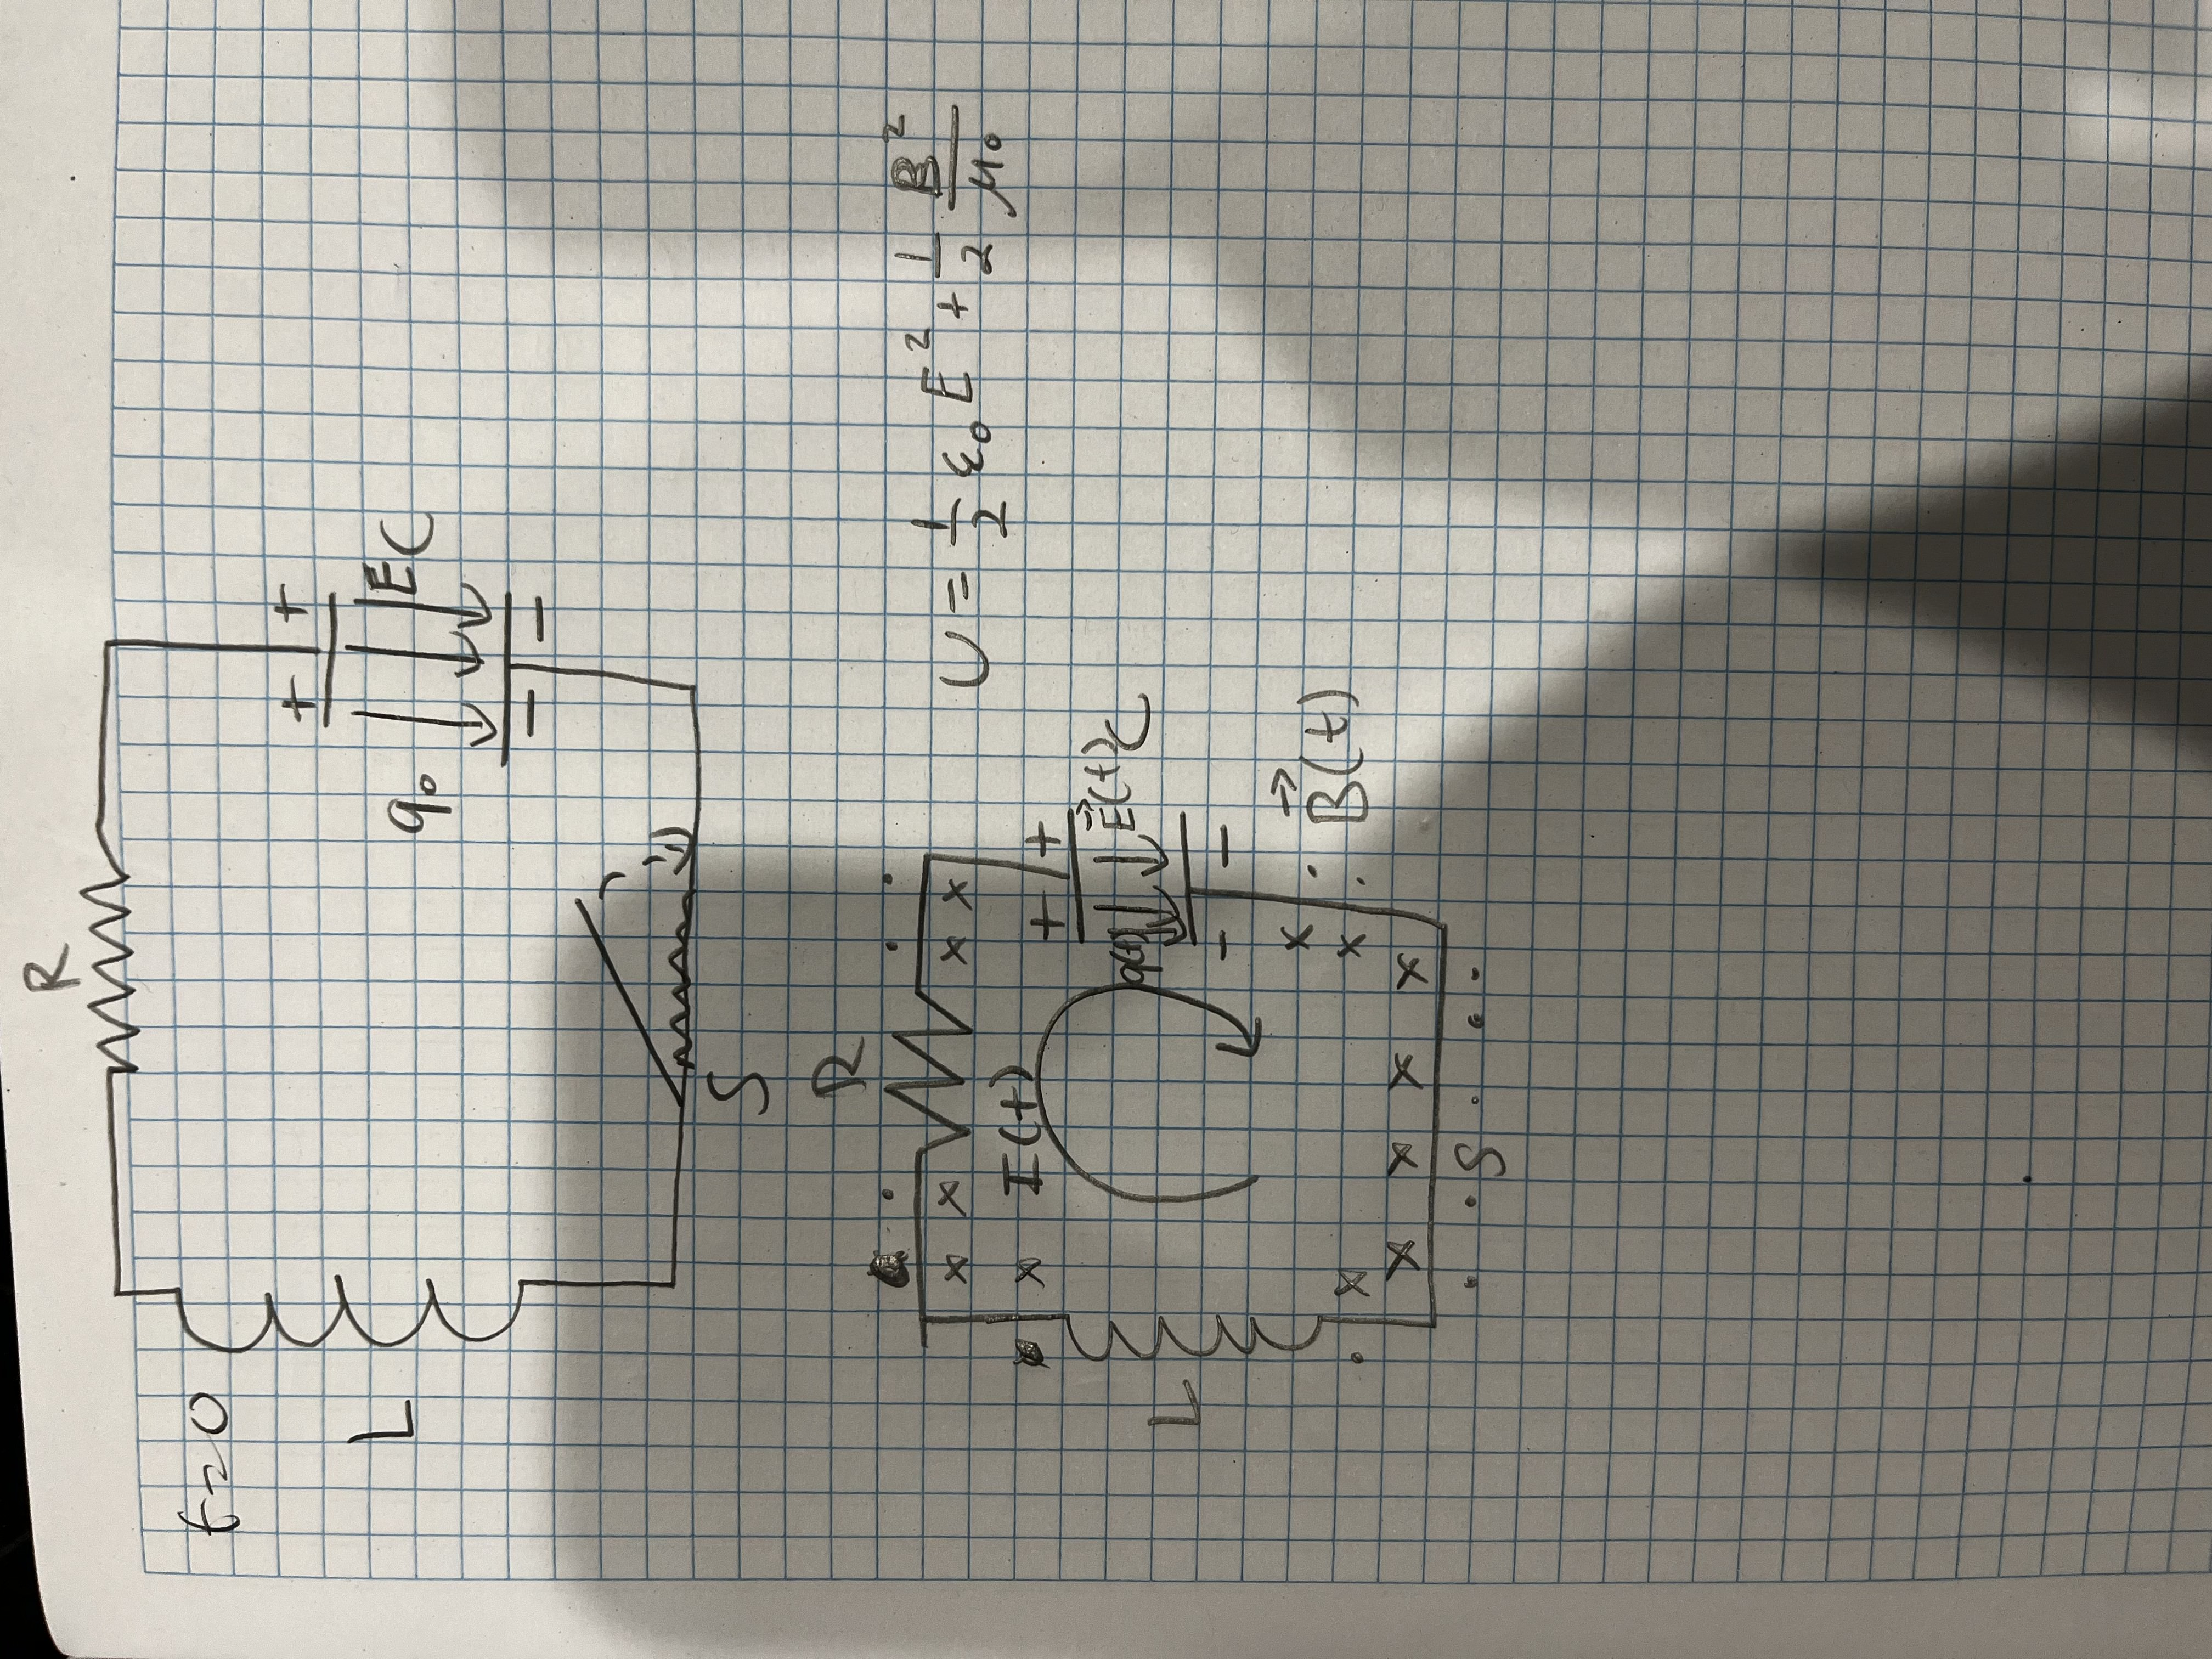
\includegraphics[width=1\textwidth,angle=270]{q1.jpg}
\end{figure}
\subsubsection{Question 2}
Consider Ampere's Law,
\begin{equation}
    \oint{B\cdot ds} = \mu_0I_{enc}.
\end{equation}

Using Figure \ref{fig:diagram2} below, the LHS of Eqn. (44)
can be rewritten as the sum of each constituent,

\begin{figure}[H]
    \centering
    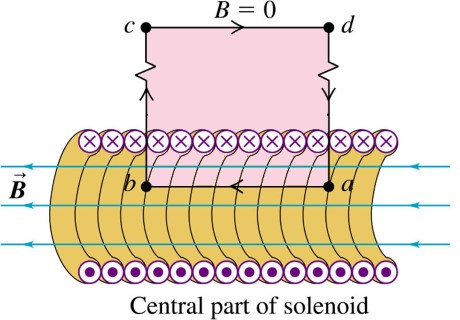
\includegraphics[width=0.5\textwidth]{diagram1.jpeg}
    \label{fig:diagram2}
\end{figure}

\begin{equation}
    \oint{B\cdot ds} = (Bl)_{ab} + (Bl)_{bc} + (Bl)_{cd} + 
    (Bl)_{da}
\end{equation}
where l is the length of the solenoid.

From Figure \ref*{fig:diagram2}, it can be seen that 
$\vec{BC}$ and $\vec{DA}$ are perpendicular to the magnetic
field and $\vec{CD}$ is outside of the solenoid 
($\vec{B}_{inside} \gg \vec{B}_{outside}$) so they will
all result in a $\vec{B}$ field of 0.

Hence,
\begin{equation}
    Bl = \mu_0 I_{enc}
\end{equation}

The current enclosed is simply the number of coils multiplied
by the current going through the solenoid so,

\begin{equation}
    B = \frac{\mu_0 N I}{l}.
\end{equation}

THe inductance of the coil is the ratio between its magnetic
flux linkage and the current that generated it,
\begin{equation}
    L = \frac{N\Phi_{B}}{I}.
\end{equation}

The magnetic flux in the solenoid is the magnetic field 
multiplied by the area of the cross section of the solenoid,

\begin{equation}
    \begin{split}
        \Phi_B &= B \cdot A \\
        &= B \pi \left(\frac{D}{2}\right)^2
    \end{split}
\end{equation}

where D is the diameter of solenoid. Let d denote the diameter 
of the wire used, so $N = \frac{l}{d}$. Combining all equations,

\begin{equation}
    \begin{split}
        L &= \frac{N(\mu_0NI)(\pi D^2)}{4lI} \\
        &= \frac{N^2\mu_0\pi D^2}{4l} \\
        &= \frac{\mu_0 \pi D^2 (l^2)}{4l (d^2)} \\
        &= \frac{\mu_0 \pi l}{4} \left(\frac{D}{d}\right)^2.
    \end{split}
\end{equation}

\subsubsection{Question 3}
Substituting the values into Eqn. (50),
\begin{equation}
    \begin{split}
        L &= \frac{\mu_0 \pi l}{4} \left(\frac{D}{d}\right)^2 \\
        &= \frac{(4\pi \times 10^{-7})(\pi)(110\times 10^{-3})}
        {4}\left(\frac{82.5\times 10^{-3}}{0.5 \times 10^{-3}}\right)^2 \\
        &= 0.00295569977\dots \\
        &\approx 2.96 \: mH
    \end{split}
\end{equation}
\subsubsection{Question 4}
The resonant frequency is calculated using Eqn. (27),
\begin{equation}
    \omega_0  = \frac{1}{\sqrt{LC}}.
\end{equation}

Substituting in L = 2.56 mH and C = 47 nF,

\begin{equation}
    \begin{split}
    \omega_0 &= \frac{1}{\sqrt{(2.56\times 10^{-3})(47\times 10^{-9})}} \\
    &= 91166 rads^{-1}.    
    \end{split}
\end{equation}

The Q-factor can be calculated using Eqn. (29)
\begin{equation}
    Q = \frac{1}{R}\sqrt{\frac{L}{C}}.
\end{equation}

Substituting in L = 2.56 mH, R = 12 $\Omega$ and C = 47 nF,

\begin{equation}
    \begin{split}
        Q &= \frac{1}{12}\sqrt{\frac{2.56 \times 10^{-3}}{47\times 10^{-9}}} \\
        &= 19.45.
    \end{split}
\end{equation}

To find bandwidth, Eqn. (37) is used,
\begin{equation}
    \begin{split}
        Q &= \frac{\omega_0}{|\Delta\omega|} \\
        |\Delta\omega| &= \frac{\omega_0}{Q}. 
    \end{split}
\end{equation}

Substituting the previous two values,
\begin{equation}
    \begin{split}
        |\Delta\omega| &= \frac{91166}{19.45} \\
        &= 4687.2 \: rads^{-1}.
    \end{split}
\end{equation}

\subsection{Pre-Work: Experimental}
\subsubsection{Question 1}
The capacitor is charged when the high state of the square wave is inputted
and discharged at low state square waves inputs. When the capacitor is fully
charged, the current through the circuit will stop, mimicking an open circuit.
When the capacitor is not fully charged, a current will flow through the resistor
and inductor. The oscillating charging and discharging will mimic the oscillatory
transient response of the circuit in Figure 2.

\subsubsection{Question 2}
Since the input is an AC signal, the voltage polarity will switch periodically, 
meaning the capacitor will charge and discharge in both directions. The diode 
will ensure that the charging and discharging cycle of the capacitor only occurs 
in one direction, mimicking the closing and opening of a switch with a circuit
with a DC voltage source like a battery.

\subsubsection{Question 3}
The oscilloscope is connected across the capacitor to read its voltage directly.
The capacitor is chosen over the resistor or inductor because it is the most 
efficient at storing energy, giving a better indicator of the circuit's dynamics.
Inductors store their energy in magnetic fields, making readings more volatile due to
magnetic flux linkage not being efficient and resistors dissipate energy as heat, 
dropping the voltage more than desired.

\subsubsection{Question 4}
The decay trace of the circuit happens over time so the oscilloscope is helpful as 
it measures periodic signals. It can accurately display rapid chagnes in voltage 
over time, allowing for precise visualisation of the transient oscillations and their
decay.

\subsubsection{Question 5}
The 160 Hz AC signal may not necessarily have anything to do with the resonant frequency
or damping constant which is both determined by the resistance, inductance and capacitance
of the circuit. Any frequency can be used to probe the dynamics of the transient response.

\subsubsection{Question 6}
Since the input voltage is at resonant frequency, $V_L =V_C$, and reactance is zero 
so the only component of impedance is resistance. This means that each of the components' 
voltage drop is proportional to their resistance. The circuit is ideal meaning the resistance
of the inductor and capacitor is zero.

To satisfy Kirchhoff's law,
\begin{equation}
    \begin{split}
    V_{in} &= V_R + V_L + V_C \\
    &= V_R + 2V_L \\
    &= V_R + 2(0) \\
    &= V_R.
    \end{split}
\end{equation}

\subsubsection{Question 7}
Off-resonant sine waves will decrease the ratio as the voltage drops of the capacitor and 
inductor becomes non-zero.

\subsubsection{Question 8}
On resonance, since the resistance of the inductor and capacitor is zero, the only form of 
energy losses will be from the resistor. Off resonance, the main energy loss components will
be from the inductor, from its wire resistance, and the capacitor's dielectric losses.

\subsubsection{Question 9}
The wires connecting the components, the wires in the inductor, diode, capacitor, resistor. 
Most of these are negligible because the voltage is being measured at the capacitor so only
the resistance of the inductor and capacitor really matters.

\subsubsection{Question 10}
By changing the frequency of the signal, the amplitude of the signal will change, producing 
some resonance curve. However, since the signal generator will output a non-constant amplitude,
the amplitude measurement could be taken as the average of the highest amplitude value and the 
lowest. You could also increase or decrease the damping of the circuit i.e change the resistance 
or inductance of the circuit to produce different curves for the resonant frequency.

\subsection{Raw Data}
\subsubsection{Transient Response}
\begin{table}[H]
    \centering
    \begin{tabular}{c|c|c}
    n & nT - $t_0$ ($\mu s$) & Voltage (V) \\
    \hline
    0	&9&	5.6 \\
    1	&145&	4.2 \\
    2	&228&	3.4 \\
    3	&304&	2.6 \\
    4	&380&	2 \\
    5	&460&	1.6 \\
    6	&540&	1.2 \\
    7	&616&	1 \\
    8	&696&	0.6 \\
    9	&776&	0.4 \\
    10	&852&	0.2
    \end{tabular}
    \caption{Raw data for Figure \ref{fig:plot1}.}
    \label{fig:t1}
\end{table}
\subsubsection{Steady State Response}
\begin{table}[H]
    \centering
    \begin{tabular}{c|c}
        Frequency (kHz) & Voltage (V) \\
        \hline
        10	&	2.74	\\
        11	&	3.536	\\
        12	&	4.582	\\
        13	&	4.814	\\
        14	&	3.675	\\
        15	&	2.593	\\
        16	&	1.902	
    \end{tabular}
    \caption{Raw data for the Fast sweep, Figure \ref{fig:plot2}.}
    \label{fig:t2}
\end{table}
\begin{table}[H]
    \centering
    \begin{tabular}{c|c|c|c}
        Frequency (kHz) & Input Voltage (V) & Voltage over resistor (V) &
        $\Delta t$ ($\mu s$) \\
        \hline
        10	&	1.071	&	41.9	&	-22.4	\\
        10.25	&	1.048	&	45.5	&	-21.6	\\
        10.5	&	1.02	&	49.5	&	-23.2	\\
        10.75	&	0.984	&	53.9	&	-21.6	\\
        11	&	0.94	&	58.8	&	-20.8	\\
        11.25	&	0.883	&	64.2	&	-19.2	\\
        11.5	&	0.814	&	69.9	&	-17.6	\\
        11.75	&	0.728	&	75.8	&	-16	\\
        12	&	0.626	&	81.5	&	-14.4	\\
        12.25	&	0.522	&	86.6	&	-12.6	\\
        12.5	&	0.409	&	90.5	&	-10.4	\\
        12.75	&	0.33	&	92.6	&	-5.6	\\
        13	&	0.329	&	92.6	&	2.4	\\
        13.25	&	0.404	&	90.6	&	8.8	\\
        13.5	&	0.509	&	87.2	&	11.2	\\
        13.75	&	0.613	&	82.8	&	12.8	\\
        14	&	0.694	&	77.9	&	15.2	\\
        14.25	&	0.771	&	73	&	13.6	\\
        14.5	&	0.835	&	68.1	&	12.8	\\
        14.75	&	0.887	&	63.7	&	14.4	\\
        15	&	0.93	&	59.6	&	14.4	\\
        15.25	&	0.965	&	55.9	&	14.4	\\
        15.5	&	0.993	&	52.5	&	14.4	\\
        15.75	&	1.017	&	49.4	&	12.8	\\
        16	&	1.036	&	46.6	&	12.8	
    \end{tabular}
    \caption{Raw data for Figure \ref{fig:plot3}.}
    \label{fig:t3}
\end{table}
\begin{table}[H]
    \centering
    \begin{tabular}{c|c|c|c}
        Frequency (kHz) & Input Voltage (V) & Voltage over resistor (V) &
        $\Delta t$ ($\mu s$) \\
        \hline
        11.9	&	0.667	&	79.8	&	-15.2	\\
        12	&	0.624	&	82	&	-15.2	\\
        12.1	&	0.58	&	84.1	&	-15.2	\\
        12.2	&	0.544	&	86.1	&	-14.4	\\
        12.3	&	0.497	&	88	&	-13.6	\\
        12.4	&	0.45	&	89.6	&	-11.2	\\
        12.5	&	0.407	&	90.9	&	-10.4	\\
        12.6	&	0.369	&	92	&	-8.8	\\
        12.7	&	0.339	&	93	&	-6.4	\\
        12.8	&	0.321	&	93	&	-3.2	\\
        12.9	&	0.318	&	93	&	0	\\
        13	&	0.329	&	93	&	2.4	\\
        13.1	&	0.353	&	92	&	4.8	\\
        13.2	&	0.386	&	92	&	8.8	\\
        13.3	&	0.425	&	90	&	9.6	\\
        13.4	&	0.467	&	89	&	10.4	\\
        13.5	&	0.51	&	87	&	11.2	\\
        13.6	&	0.552	&	86	&	12.8	\\
        13.7	&	0.594	&	84	&	12.8	\\
        13.8	&	0.634	&	82	&	12.8	\\
        13.9	&	0.659	&	80	&	12.8	    
    \end{tabular}
    \caption{Raw data for Figure \ref{fig:plot4}}
    \label{fig:t4}
\end{table}
\begin{table}[H]
    \centering
    \begin{tabular}{c|c|c|c}
        Frequency (kHz) & Input Voltage (V) & Voltage over resistor (V) &
        $\Delta t$ ($\mu s$) \\
        \hline
        11.9	&	0.674	&	19.2	&	-18.4	\\
        12	&	0.628	&	19.9	&	-16.8	\\
        12.1	&	0.579	&	20.5	&	-16	\\
        12.2	&	0.538	&	21.1	&	-16	\\
        12.3	&	0.484	&	21.6	&	-14.4	\\
        12.4	&	0.43	&	22	&	-13.6	\\
        12.5	&	0.378	&	22.4	&	-12	\\
        12.6	&	0.33	&	22.7	&	-8.8	\\
        12.7	&	0.291	&	22.9	&	-7.2	\\
        12.8	&	0.267	&	22.9	&	-4.8	\\
        12.9	&	0.262	&	22.9	&	0	\\
        13	&	0.278	&	22.8	&	4.8	\\
        13.1	&	0.31	&	22.6	&	5.6	\\
        13.2	&	0.352	&	22.4	&	10.4	\\
        13.3	&	0.4	&	22	&	9.6	\\
        13.4	&	0.45	&	21.7	&	10.4	\\
        13.5	&	0.499	&	21.2	&	11.2	\\
        13.6	&	0.548	&	20.7	&	12	\\
        13.7	&	0.594	&	20.1	&	12	\\
        13.8	&	0.637	&	19.6	&	13.6	\\
        13.9	&	0.666	&	19	&	14.4	
    \end{tabular}
    \caption{Raw data for Figure \ref{fig:plot5}}
    \label{fig:t5}
\end{table}
\begin{table}[H]
    \centering
    \begin{tabular}{c|c|c|c}
        Frequency (kHz) & Input Voltage (V) & Voltage over resistor (V) &
        $\Delta t$ ($\mu s$) \\
        \hline
        11.9	&	0.665	&	147.7	&	-14.4	\\
        12	&	0.626	&	151.5	&	-14.4	\\
        12.1	&	0.587	&	155	&	-12.8	\\
        12.2	&	0.547	&	158.2	&	-11.2	\\
        12.3	&	0.518	&	161.2	&	-10.4	\\
        12.4	&	0.48	&	163.7	&	-9.6	\\
        12.5	&	0.446	&	165.9	&	-8	\\
        12.6	&	0.416	&	167.6	&	-6.4	\\
        12.7	&	394.4	&	168.8	&	-4	\\
        12.8	&	0.382	&	169.5	&	-2.4	\\
        12.9	&	0.379	&	169.6	&	0	\\
        13	&	0.387	&	169.2	&	3.2	\\
        13.1	&	0.404	&	168.3	&	4.8	\\
        13.2	&	0.429	&	167	&	6.4	\\
        13.3	&	0.459	&	165.2	&	6.4	\\
        13.4	&	0.492	&	163.1	&	8	\\
        13.5	&	0.528	&	160.7	&	9.6	\\
        13.6	&	0.564	&	158	&	11.2	\\
        13.7	&	0.599	&	155	&	11.2	\\
        13.8	&	0.634	&	152	&	12	\\
        13.9	&	0.656	&	148.8	&	10.4	    
    \end{tabular}
    \caption{Raw data for Figure \ref{fig:plot6}}
    \label{fig:t6}
\end{table}
\subsection{Lab Book}
\begin{figure}[H]
    \centering
    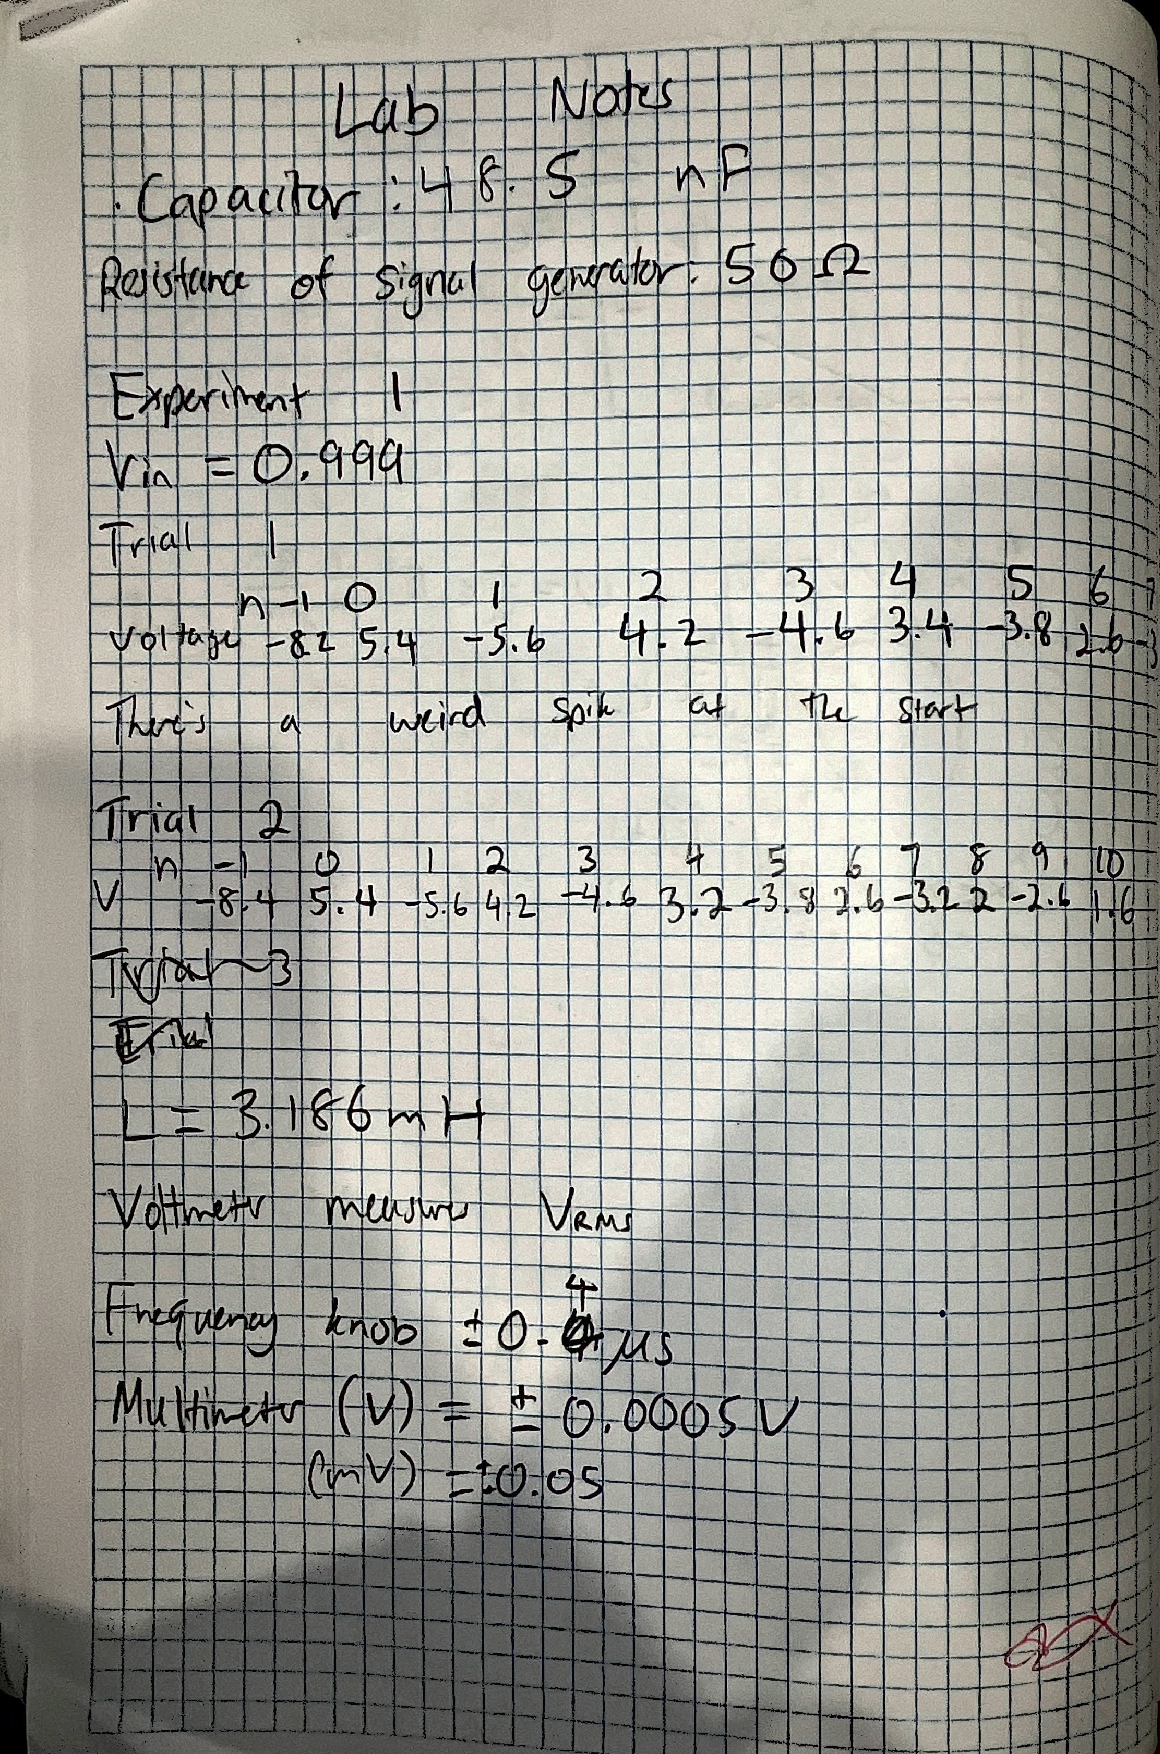
\includegraphics[width=0.8\textwidth]{labbook.pdf}
\end{figure}
\end{document}